\documentclass[twoside]{article}
%\usepackage{aistats2018}
 % If your paper is accepted, change the options for the package
% aistats2018 as follows:
%
\usepackage[accepted]{aistats2018}
%
% This option will print headings for the title of your paper and
% headings for the authors names, plus a copyright note at the end of
% the first column of the first page.

\usepackage[compress,round]{natbib}
\usepackage{amsmath,amssymb,amsfonts,amsthm,amscd,bm,bbm}
\usepackage{mathtools}
\mathtoolsset{showonlyrefs}
\usepackage[inline]{enumitem}
\usepackage[inline]{enumitem}
\usepackage[pdftex]{graphicx}
\graphicspath{{./figs/}}
\usepackage{algorithmic}
\usepackage{algorithm}
\usepackage{multirow}
\usepackage{colortbl}
\usepackage{array,booktabs}
\usepackage{xcolor}
\usepackage{makecell}
\usepackage{pifont}
\newcommand{\cmark}{\ding{51}}
\newcommand{\xmark}{\ding{55}}

\newtheorem{theorem}{Theorem}
\newtheorem{definition}[theorem]{Definition}
\newtheorem{assumption}[theorem]{Assumption}
\newtheorem{lemma}[theorem]{Lemma}
\newtheorem{corollary}[theorem]{Corollary}
\newtheorem{proposition}[theorem]{Proposition}
\newtheorem{conjecture}[theorem]{Conjecture}
\newtheorem{remark}[theorem]{Remark}
\newtheorem{example}{Example}

\DeclareMathOperator{\aff}{aff}
\DeclareMathOperator{\st}{s.t.}
\DeclareMathOperator{\affnot}{aff_0}
\DeclareMathOperator{\conv}{conv}
\DeclareMathOperator{\relint}{relint}
\DeclareMathOperator{\vol}{vol}
\DeclareMathOperator{\range}{range}
\DeclareMathOperator{\image}{im}
\DeclareMathOperator{\nullspace}{null}
\DeclareMathOperator{\area}{area}
\DeclareMathOperator{\vspan}{span}
\DeclareMathOperator{\id}{Id}
\DeclareMathOperator{\cond}{cond}
\DeclareMathOperator{\prox}{prox}
\DeclareMathOperator*{\argmax}{arg\,max}
\DeclareMathOperator*{\argmin}{arg\,min}
\DeclareMathOperator*{\minimize}{minimize}
\DeclareMathOperator{\diag}{diag}
\DeclareMathOperator{\Tr}{Tr}

\newcommand\Energy{\mathcal{E}}
\newcommand\EnergyH{\mathcal{E}^{H}}
\newcommand\EnergyL{\mathcal{E}^{L}}
\newcommand\EnergyOne{\mathcal{E}^{1D}}
\newcommand\E{\mathbb{E}}
\newcommand\kk{K}
\newcommand\kkk{h}
\newcommand\Hk{{\mathcal{H}}_{\kk}}
\newcommand\HH{\mathcal{H}}
\newcommand\C{{\mathcal{C}}}
\newcommand\tC{{\widetilde{\C}}}
\newcommand\OO{{\mathcal{O}}}
\newcommand\Zt{Y}
\newcommand{\Ind}[1]{\mathbbm{1}_{#1}}
\newcommand\e{e}
\newcommand\om{\omega}
\newcolumntype{g}{>{\columncolor{gray!20}}l}



\begin{document}

% If your paper is accepted and the title of your paper is very long,
% the style will print as headings an error message. Use the following
% command to supply a shorter title of your paper so that it can be
% used as headings.
%
%\runningtitle{I use this title instead because the last one was very long}

% If your paper is accepted and the number of authors is large, the
% style will print as headings an error message. Use the following
% command to supply a shorter version of the authors names so that
% they can be used as headings (for example, use only the surnames)
%
%\runningauthor{Surname 1, Surname 2, Surname 3, ...., Surname n}

\twocolumn[

\aistatstitle{Clustering via Generalized Energy Statistics}

\aistatsauthor{Guilherme Fran\c{c}a \And  Joshua T. Vogelstein}

\aistatsaddress{ Johns Hopkins University } ]

\begin{abstract}
Energy statistics introduces the notion of potential
energy between probability distributions, in  
close analogy to Newton's gravitational
potential in physics. We propose a principled approach to the
clustering problem based on energy statistics theory.
Our mathematical formulation establishes connection to kernel methods,
leading to a quadratically constrained quadratic program (QCQP).
To obtain local solutions of such NP-hard QCQP 
we introduce an iterative
algorithm based
on Hartigan's method, which has the same computational cost but offers
several advantages compared to  
kernel $k$-means, based on Lloyd's heuristic.
We provide carefully designed numerical experiments showing
that our method is more flexible and outperforms
kernel $k$-means, spectral clustering,
standard $k$-means and Gaussian mixture models in a variety of settings,
specially in high dimensions. 
\end{abstract}


%%%%%%%%%%%%%%%%%%%%%%%%%%%%%%%%%%%%%%%%%%%%%%%%%%%%%%%%%%%%%%%%%%%%%%%%%%%%%%%
\section{Introduction}

Energy statistics \citep{Szkely2013}
provides a hypothesis test for equality of 
distributions which is achieved 
under minimum statistical potential energy. 
When probability distributions are different the 
statistical potential energy diverges as sample size increases, while tends 
to a nondegenerate limit distribution when probability
distributions are equal. 
The test statistic has compact representation
in terms of expectations of pairwise distances, providing
straightforward empirical estimates. Energy statistics
has been applied to several goodness-of-fit 
hypothesis tests, multi-sample tests of equality of distributions, 
analysis of variance \citep{RizzoVariance}, nonlinear dependence tests through
distance covariance and distance correlation, which generalizes the Pearson
correlation coefficient, and hierarchical clustering \citep{RizzoClustering} 
by extending Ward's method of minimum variance. Moreover, an application of 
energy statistics to clustering, in Euclidean spaces, was 
proposed \citep{Kgroups}, which in part motivated this paper. 
We refer to \citep{Szkely2013} for an overview.

Distance covariance was further generalized from Euclidean 
to metric spaces of strong negative type \citep{Lyons}. Furthermore, 
the missing link between energy distance based tests and kernel 
based tests has 
been recently resolved \citep{Sejdinovic2013}, where a unifying framework
establishing an equivalence between generalized energy distances to maximum
mean discrepancies (MMD), which are distances between embeddings of 
distributions in reproducing kernel Hilbert spaces (RKHS), was established. 
This equivalence immediately relates energy statistics to
kernel methods often used in machine learning, and form the basis 
of our approach.

Clustering has such a long history in machine learning, making it
impossible to mention all important contributions in a short space. 
Perhaps, the most used method is $k$-means \citep{Lloyd,MacQueen,Forgy}, which
is based on Lloyd's heuristic \citep{Lloyd} of assigning a data point to
the cluster with closest center. The only statistical 
information about each cluster comes from its mean, making it sensitive 
to outliers. Nevertheless, $k$-means works very well when data is 
linearly separable in Euclidean space. Gaussian mixture models (GMM) is 
another very common approach, providing more flexibility than $k$-means, 
however, it still makes strong assumptions about the distribution of 
the data.

To account for nonlinearities, kernel methods were introduced 
\citep{Smola,Girolami}. A mercer kernel \citep{Mercer} is used to implicitly
map data points to a RKHS, then clustering can be performed in the associated
Hilbert space by exploiting its inner product. However, the kernel choice remains 
the biggest challenge since there is no principled theory to construct a kernel
for a given dataset, and usually kernels introduce hyperparameters that 
need to be carefully chosen.
The well-known kernel $k$-means optimization problem is nothing but $k$-means 
in the feature space \citep{Girolami}. Furthermore, kernel $k$-means algorithm
\citep{Dhillon2,Dhillon} is still based on Loyd's heuristic \citep{Lloyd}
of grouping points that are closer to a cluster center, now
in feature space. 
We refer the reader to \citep{Filippone} for a survey of clustering
methods.

Although clustering from energy statistics in Euclidean spaces was considered
in \citep{Kgroups}, the precise optimization problem behind this approach
remains elusive, as well as the connection with kernel methods.
The main theoretical contribution of this paper is to fill this gap.
Since the statistical potential energy is minimum when
distributions are equal, the principle behind clustering is to maximize 
the statistical energy,  enforcing probability distributions associated to 
each cluster to be different from one another. We provide a precise 
mathematical formulation to this statement, leading to a quadratically 
constrained quadratic program (QCQP) in the associated RKHS. Our results
immediately establish the connection with kernel methods, showing that this 
QCQP is equivalent to kernel $k$-means optimization problem. 

Our main 
algorithmic contribution is to use Hartigan's method \citep{Hartigan} to 
find local solutions of the above mentioned QCQP, which is NP-hard in general.
Hartigan's method was also used in \citep{Kgroups}, without any
connection to kernels. More importantly, its 
advantages
over Lloyd's method was already demonstrated 
in some simple settings
\citep{Telgarsky,Slonin}, but apparently this method did not receive 
the deserved attention. To the 
best of our knowledge, Hartigan's method was not previously 
employed together with kernel methods. 
We provide a full kernel based Hartigan's algorithm for clustering,
where the kernel is fixed by energy statistics. 
We make clear the advantages of this proposal versus 
Lloyd's method, which kernel $k$-means is based upon and will also be used 
to solve our QCQP. We show that both algorithms  have the same
time complexity, but Hartigan's method in kernel spaces offer several
advantages. Furthermore, in the examples considered in this paper, it 
also provides superior performance compared to a spectral clustering.
Our numerical results provide compelling evidence that 
Hartigan's method applied to energy statistics based clustering
is more accurate and robust than 
kernel $k$-means. Moreover, we illustrate the
flexibility of energy clustering,  
showing that it is able to perform accurately on data coming from 
different distributions, contrary to $k$-means and GMM for instance.
The proposed algorithm performs 
closely to $k$-means and GMM on normally distributed data, however,
it is significantly better on other settings. 
Its superiority in high dimensions is striking, being more accurate 
than $k$-means and GMM even on Gaussian settings.


%%%%%%%%%%%%%%%%%%%%%%%%%%%%%%%%%%%%%%%%%%%%%%%%%%%%%%%%%%%%%%%%%%%%%%%%%%%%%%%
\section{Background}
\label{sec:background}

In this section we introduce the main concepts from (generalized) energy
statistics \citep{Szkely2013,Lyons} and its relation to 
RKHS \citep{Sejdinovic2013}
which form the basis of our work.

Consider random vectors $X_i$ living in an arbitrary space
$\mathcal{X}$ of \emph{negative type}, which means that $\mathcal{X}$
is endowed with a \emph{semimetric} 
$\rho: \mathcal{X}\times\mathcal{X} \to \mathbb{R}$ satisfying
$\sum_{i,j=1}^n c_i c_j \rho(X_i, X_j) \le 0$,
where $c_i \in \mathbb{R}$ and
$\sum_{i=1}^n c_i = 0$. 
Let $X,X' \stackrel{iid}{\sim} P$ and 
$Y,Y' \stackrel{iid}{\sim} Q$, where $P$ and $Q$ are cumulative
distribution functions with finite first moments, and 
$X,X',Y,Y' \in \mathcal{X}$. 
The \emph{generalized energy distance} between $P$ and $Q$ is
given by 
\begin{equation}
\label{eq:energy3}
\Energy(P, Q) \equiv 2 \E \rho(X,Y) - \E \rho(X, X') - \E \rho(Y,Y').
\end{equation} 
This quantity is nonnegative, $\Energy(P,Q) \ge 0$, and 
$\Energy^{1/2}$ is
a metric on the space of distributions. Energy distance provides
a characterization of equality of distributions.

For instance, the \emph{standard
energy distance} \citep{Szkely2013} in Euclidean spaces uses
the semimetric
\begin{equation}
\label{eq:rho_standard}
\rho_\alpha(X,Y) = \| X - Y\|^\alpha,
\end{equation} 
where $0< \alpha \le 2$ and $\| \cdot \|$ is the
Euclidean norm in $\mathcal{X}=\mathbb{R}^D$. In this case $\Energy(P,Q)$
is rotationally invariant. For $0<\alpha<2$ we have
$\Energy(P,Q) = 0$ if and only if $P=Q$. However, for $\alpha=2$
we get $\Energy(P,Q) = 2\| \E(X) - \E(Y) \|^2$, thus
$\Energy(P,Q)=0$ does 
not imply equality of distributions but only equality
of the means.
 
Consider data $\mathbb{X} = \{ x_1,\dotsc, x_n \}$ 
sampled from $k$ unknown distributions $\{ P_j \}_{j=1}^k$,
with points lying on a space of negative type,
$x_i \in \mathcal{X}$.
Let $\mathbb{X} = \bigcup_{j=1}^k \C_j$ be a disjoint
partition, $\C_i \cap \C_j = \emptyset$.
Each expectation in the generalized energy distance
can be empirically estimated with the aid of the
function
\begin{equation}
\label{eq:g_def}
g (\C_i, \C_j) \equiv 
\dfrac{1}{n_i n_j}
\sum_{x \in \C_i} 
\sum_{y \in \C_j} \rho(x, y) ,
\end{equation}
where $n_i = |\C_i|$ is the number of elements in partition
$\C_i$. 
Define the \emph{within energy dispersion} as
\begin{equation}
\label{eq:within}
W \equiv
\sum_{j=1}^{k} \dfrac{n_j}{2} g(\C_j, \C_j),
\end{equation}
and the \emph{between-sample energy statistic} as
\begin{equation}
\label{eq:between}
S \equiv \hspace{-1em}
\sum_{1 \le  i < j \le k } \hspace{-.5em} \dfrac{n_i n_{j}}{2 n} \left[
2 g(\C_i, \C_j) - 
g(\C_i, \C_i) - 
g(\C_j, \C_j)
\right],
\end{equation}
where $n = \sum_{j=1}^k n_j$.
A given point $x_i$ belongs to partition $\C_j$
if and only if $x_i \sim P_j$. 
The quantity $S$ is
a test statistic for equality of distributions
\citep{Szkely2013}.
When the sample size is large enough, $n\to \infty$,
under the null hypothesis $H_0: P_1=P_2=\dotsm=P_k$ we have that
$S\to 0$, 
and under
the alternative hypothesis $H_1: P_\ell \ne P_j$ for at least two $\ell\ne j$, 
we have that $S \to \infty$.

Let $\HH_\kk$ be a Hilbert space of real-valued functions
over $\mathcal{X}$ with an associated kernel
$\kk : \mathcal{X} \times \mathcal{X} \to 
\mathbb{R}$, which is a symmetric and positive definite function, i.e. 
$\kk(x_i,x_j) = \kk(x_j,x_i)$ and 
$\sum_{i,j=1}^n c_i c_j \kk(x_i, x_j) \ge 0$, or equivalently,
if $G$ is the Gram matrix with entries $G_{ij} = \kk(x_i,x_j)$
then $G = G^\top$ and $v^\top G v \ge 0$ for any $v \in \mathbb{R}^n$.
For every $x \in \mathcal{X}$ there exists 
$h_x \equiv \kk(\cdot,x) \in \Hk$ such that  $\langle h_x, f \rangle = f(x)$
for any function $f \in \Hk$. Thus, 
$\langle h_x, h_y \rangle = \kk(x,y)$.
Conversely \citep{Aronszajn},  
for every symmetric
positive definite function $\kk: \mathcal{X}\times \mathcal{X} \to
\mathbb{R}$ there is a Hilbert space $\Hk$ with reproducing
kernel $\kk$, with a 
\emph{feature map} $\varphi: x \mapsto \kkk_x \in \Hk$ such
that $\langle \varphi(x), \varphi(y) \rangle = \kk(x, y)$.

Define the embedding of a probability measure
$P \mapsto \kkk_P \in \Hk$ through
$\kkk_P \equiv \int \kk( \, \cdot \,, x)  d P(x)$. 
The distance between two probability measures, 
called maximum mean discrepancy (MMD), is thus given by
\begin{equation}
\label{eq:mmd}
\gamma_\kk(P,Q) \equiv \| \kkk_P - \kkk_Q \|_{\Hk},
\end{equation}
which can also be written as \citep{Gretton2012}
\begin{equation}\label{eq:mmd2}
\gamma_\kk^2(P,Q) = \E \kk(X,X') + \E \kk(Y,Y') - 2 \E \kk(X, Y)
\end{equation}
where $X,X' \stackrel{iid}{\sim} P$ and $Y,Y'\stackrel{iid}{\sim} Q$.
The equality between \eqref{eq:mmd} and \eqref{eq:mmd2}
gives $\langle \kkk_P, \kkk_Q \rangle_{\Hk} = \E \, \kk(X, Y)$,
thus in practice we can estimate the inner product between  
embedded distributions by averaging the kernel function over sampled data.

The following important result shows that semimetrics of negative
type and symmetric positive definite kernels are closely related
\citep{Berg1984}. Let $\rho: \mathcal{X} \times \mathcal{X} \to \mathbb{R}$
and $x_0 \in \mathcal{X}$ an arbitrary but fixed point.
Define
\begin{equation}
\label{eq:kernel_semimetric}
\kk(x,y) \equiv 
\tfrac{1}{2} \left[  \rho(x,x_0) + \rho(y,x_0) - \rho(x,y)\right].
\end{equation}
Then, it can be shown that 
$\kk$ is positive definite if and only if $\rho$ is a semimetric
of negative type.
We have a family of kernels, one for each choice of $x_0$. Conversely,
if $\rho$ is a semimetric of negative type and $\kk$ is a kernel in this
family, then 
\begin{equation}
\label{eq:gen_kernel}
\begin{split}
\rho(x,y) &= \kk(x,x) + \kk(y,y) -2\kk(x,y) \\
&=  \| \kkk_x - \kkk_y \|^2_{\Hk}
\end{split}
\end{equation}
and the canonical feature map 
$\varphi: x \mapsto \kkk_x$ is injective \citep{Sejdinovic2013}.
When these conditions are satisfied we say that the kernel $\kk$ 
generates the semimetric $\rho$. 
If two different kernels generate the same $\rho$ they are
said to be equivalent kernels.
Now we can state the equivalence between energy distance and
inner products on RKHS, which is one of the main results of
\citep{Sejdinovic2013}. If $\rho$ is a semimetric
of negative type and $\kk$ a kernel that generates $\rho$, then
replacing \eqref{eq:gen_kernel} into
\eqref{eq:energy3}, and using \eqref{eq:mmd2}, yields
\begin{equation}
\label{eq:Erho}
\begin{split}
\tfrac{1}{2}\Energy(P, Q) &= 
\E \, \kk(X, X') + \E \, \kk(Y, Y') - 2\E \, \kk(X, Y) \\ 
&= \gamma_\kk^2(P,Q) ,
\end{split}
\end{equation}
so we can compute the energy distance using the inner product
of $\Hk$.


%%%%%%%%%%%%%%%%%%%%%%%%%%%%%%%%%%%%%%%%%%%%%%%%%%%%%%%%%%%%%%%%%%%%%%%%%%%%%%%
\section{Clustering via Energy Statistics}
\label{sec:clustering_theory}

This section contains our main theoretical results, where 
we formulate an optimization problem for clustering 
based on energy statistics in the RKHS introduced in the previous section.
The proofs are contained in supplementary material.

Due to the energy test statistic for equality of distributions,
the obvious
criterion for clustering data is to 
maximize $S$ which makes 
each cluster as different
as possible from the other ones.
In other words, given a set of points coming from different probability
distributions, the test statistic $S$ should attain a maximum when 
each point is correctly
classified as belonging to the cluster associated to its probability
distribution.
The following 
straightforward result
shows that maximizing $S$ is, however, equivalent to minimizing
$W$ which has a more convenient form.

\begin{lemma}
\label{th:minimize}
Let $\mathbb{X} = \{x_1,\dotsc,x_n\}$ where each data point
$x_i$ lives in a space $\mathcal{X}$ of negative type. 
For a fixed integer $k$,
the partition
$\mathbb{X} = \bigcup_{j=1}^k \C_j$, where $\C_i \cap C_j = \emptyset$ for
all $i\ne j$, maximizes the between-sample statistic $S$, defined
in equation \eqref{eq:between}, if and only if
\begin{equation}
\label{eq:minimize}
\min_{\C_1,\dotsc,C_k  } W(
\C_1, \dotsc, \C_k),
\end{equation}
where the within energy dispersion $W$ is defined by \eqref{eq:within}.
\end{lemma}

In the Euclidean case, the optimization problem \eqref{eq:minimize} based on
energy statistics was already proposed in \citep{Kgroups}. However, it is
important to note that this is equivalent to maximizing $S$,
which is the test statistic for equality of distributions. In this current
form, the relation with kernels and other clustering methods is obscure.
In the following, we show what is the explicit optimization problem behind 
\eqref{eq:minimize} in the corresponding RKHS, 
establishing the connection with kernel methods.

Assume that the kernel $\kk: \mathcal{X} \times \mathcal{X} \to \mathbb{R}$ 
generates $\rho$.  Define  the Gram matrix $G \in \mathbb{R}^{n\times n}$ as
\begin{equation}
\label{eq:kernel_matrix}
G_{ij} \equiv \kk(x_i,x_j).
\end{equation}
Let $Z \in \{ 0,1 \}^{n\times k}$ be the label matrix, 
with only one nonvanishing entry per row, 
indicating to which cluster (column)
each point (row) belongs to. This matrix satisfies
$Z^\top Z = D$, where  
$D = \diag( n_1,\dotsc, n_k )$  contains
the number of points in each cluster. We also introduce the rescaled
matrix  $Y \equiv Z D^{-1/2}$. In component form they are given by
\begin{equation}
\label{eq:label_matrix}
Z_{ij} \equiv \begin{cases}
1 & \mbox{if $x_i \in \C_j$ } \\
0 & \mbox{otherwise}
\end{cases} \
\Zt_{ij} \equiv \begin{cases}
\tfrac{1}{\sqrt{n_j}} & \mbox{if $x_i \in \C_j$ } \\
0 & \mbox{otherwise}
\end{cases}
\end{equation}
Throughout the paper, we use the notation $M_{i\bullet}$ to denote
the $i$th row of a matrix $M$, and $M_{\bullet j}$ denotes its $j$th column.
Our next result shows that the optimization problem \eqref{eq:minimize}
is NP-hard since
it is a quadratically constrained quadratic program (QCQP) in the RKHS.

\begin{proposition} 
\label{th:qcqp2}
The optimization problem \eqref{eq:minimize} is equivalent to
\begin{equation}
\label{eq:qcqp2}
\begin{split}
&\max_{\Zt} \Tr \left( \Zt^\top G \, \Zt \right) \\
&\mbox{s.t. $\Zt \ge 0$, $\Zt^\top \Zt = I$, 
$\Zt \Zt^\top \e = \e$},
\end{split}
\end{equation}
where $\e = (1,\dots,1)^\top \in \mathbb{R}^n$ is the all-ones vector,
and $G$ is the Gram matrix \eqref{eq:kernel_matrix}.
\end{proposition}

Therefore, to group data
$\mathbb{X} = \{ x_1,\dotsc,x_n \}$
into  $k$ clusters we first compute the Gram matrix
$G$ and then 
solve the optimization problem \eqref{eq:qcqp2} for $\Zt \in
\mathbb{R}^{n\times k}$. The $i$th row
of $\Zt$ will contain a single nonzero element in some $j$th column,
indicating that $x_i \in \C_j$. 
This optimization problem is nonconvex, and also NP-hard,
thus a direct approach 
is computational prohibitive even for small datasets.
However, one can find approximate solutions by relaxing some 
of the constraints.
For instance, the relaxed problem
$\max_{Y} \Tr \left( Y^\top G \, Y \right)$ s.t. $Y^\top Y = I$,
has a well-known closed form solution $Y^\star = U R$, where the
columns of $U \in \mathbb{R}^{n\times k}$ 
contain the top $k$ eigenvectors of $G$ corresponding
to the $k$ largest eigenvalues $\lambda_1\ge \lambda_2\ge\dotsc\ge\lambda_k$, 
and
$R \in \mathbb{R}^{k\times k}$ is an arbitrary orthogonal matrix. 
\emph{Spectral clustering} is based on (variants of) this approach 
and will be compared to the iterative method that will be proposed 
in the following.

Note that the energy clustering problem \eqref{eq:qcqp2} 
is valid for data living in an \emph{arbitrary} space of negative type, where
a semimetric $\rho$, and thus the kernel $\kk$, are
assumed to be known. Standard energy statistics in
Euclidean spaces fixes a family of choices through 
\eqref{eq:rho_standard}.
The same would be valid for data living in more general
spaces $(\mathcal{X}, \rho)$.
In any case, energy  clustering 
is model-free, 
contrary to $k$-means and GMM, for example.
In practice, however,
the clustering quality strongly depend on the choice of a suitable
$\rho$ which measures the similarity between data points.
If prior information is available to choose $\rho$
it can be conveniently incorporated in the 
optimization problem \eqref{eq:qcqp2}.

\paragraph{Relation to Kernel $\bm{k}$-Means.}
One may wonder how energy clustering 
relates to the well-known kernel $k$-means problem%
\footnote{When we refer to kernel $k$-means problem we mean specifically 
the optimization problem \eqref{eq:kernel_kmeans}, which should not be 
confused with kernel $k$-means algorithm that is just one possible recipe 
to solve \eqref{eq:kernel_kmeans}.}, 
extensively used in machine learning.
For a positive semidefinite Gram matrix $G$, as defined in
\eqref{eq:kernel_matrix},
there exists a feature map
$\varphi: \mathcal{X} \to \HH_\kk$ such that
$G_{ij} = \langle \varphi(x_i), \varphi(x_j) \rangle$. The kernel $k$-means optimization
problem,
in feature space,
is defined by
\begin{equation}
\label{eq:kernel_kmeans}
\min_{\C_1,\dotsc,\C_k}\bigg\{ 
\sum_{j=1}^k
\sum_{x \in \C_j} \| \varphi(x) - \varphi(\mu_j) \|^2
\bigg\}
\end{equation}
where $\mu_j = \tfrac{1}{n_j} \sum_{x \in \C_j} x$ is the  mean of cluster
$\C_j$ in the ambient space $\mathcal{X}$. 
Notice that the above objective function
is strongly tied to the idea of minimizing distances between points
and cluster centers, which arises from $k$-means objective function based
on Lloyd's heuristic \citep{Lloyd}.
It is known \citep{Dhillon2,Dhillon}
that kernel $k$-means problem 
can be cast into a trace maximization in the same form as 
\eqref{eq:qcqp2}. The next result makes this explicit.

\begin{proposition}
\label{th:kernel_kmeans}
For a fixed kernel,
the energy clustering optimization problem
\eqref{eq:minimize} 
is equivalent to the kernel $k$-means optimization problem
\eqref{eq:kernel_kmeans}, and both are equivalent to \eqref{eq:qcqp2}.
\end{proposition}

The above result shows that 
kernel $k$-means problem is equivalent to the clustering problem
formulated in the energy statistics framework, when operating on the same
kernel. Notice, however, that 
energy statistics theory is valid for arbitrary semimetric spaces of
negative type, fixing the kernel function in the associated RKHS, which
is guaranteed to be positive definite.
As shown by \citep{Dhillon2,Dhillon}, kernel $k$-means, spectral clustering,
and graph partitioning problems such as ratio association, ratio cut, and
normalized cut are all equivalent to a QCQP of the form \eqref{eq:qcqp2}.
Thus one can view all these problems arising from energy statistics as well.


%%%%%%%%%%%%%%%%%%%%%%%%%%%%%%%%%%%%%%%%%%%%%%%%%%%%%%%%%%%%%%%%%%%%%%%%%%%%%%%
\section{Hartigan's for Energy Clustering}
\label{sec:algo}

We introduce an iterative algorithm based
on Hartigan's method \citep{Hartigan} to find a local
maximizer of the optimization problem \eqref{eq:qcqp2}. Due to 
Proposition~\ref{th:kernel_kmeans} we can use 
kernel $k$-means algorithm \citep{Dhillon2,Dhillon}, which
will be compared with the proposed algorithm. 

We can write the optimization problem \eqref{eq:qcqp2} as
\begin{equation}
\label{eq:maxQ}
\max_{\{ \C_1,\dotsc,\C_k \}} 
\bigg\{ Q = \sum_{j=1}^k \dfrac{Q_j}{n_j}  \bigg\},
\quad Q_j \equiv \sum_{x,y\in\C_j} \kk(x,y),
\end{equation}
where $Q_j$ represents an internal energy cost of cluster $\C_j$, and
$Q$ is the total energy cost where each $Q_j$ 
is weighted by the inverse
of the number of points in $\C_j$. For a data point $x_i$ we denote
its own energy cost
with the entire cluster $\C_\ell$ by
\begin{equation}
\label{eq:costxij}
Q_\ell(x_i) \equiv \sum_{y\in\C_\ell} \kk(x_i, y) = 
G_{i \bullet} \cdot Z_{\bullet \ell},
\end{equation}
where we recall that $G_{i\bullet}$ ($G_{\bullet i}$) denotes
the $i$th row (column) of matrix $G$.

For a given configuration, we consider the maximum change
in the total cost function $Q$ when moving each data point to
another cluster. More specifically, 
suppose $x_i$
is currently assigned to  cluster $\C_j$, yielding
a total cost function denoted by $Q^{(j)}$.
Moving $x_i$ to cluster $\C_\ell$ yields another total cost function
denoted by $Q^{(\ell)}$. We are interested in computing the maximum 
cost change
$\Delta Q^{j\to \ell} (x_i) \equiv Q^{(\ell)} - Q^{(j)}$, for $\ell\ne j$. 
From \eqref{eq:maxQ}, by explicitly writing the costs related to these 
two cluster we obtain
\begin{equation}
\Delta Q^{j\to \ell} (x_i) = \dfrac{Q_\ell^{+}}{n_\ell+1} + 
\dfrac{Q_j^-}{n_j-1} - \dfrac{Q_j}{n_j} - \dfrac{Q_\ell}{n_\ell}
\end{equation}
where $Q^{+}_\ell$ denote the cost of the new $\ell$th cluster
with the point $x_i$ added to it, and $Q^-_j$ is the cost of new 
$j$th cluster with $x_i$ removed from it. Observe that 
$Q_\ell^{+} = Q_\ell + 2 Q_\ell(x_i) + G_{ii}$ and
$Q_j^{-} = Q_j - 2 Q_j(x_i) + G_{ii}$, hence
\begin{equation}
\label{eq:changeQ}
\begin{split}
\Delta Q^{j \to \ell}(x_i)  = 
\dfrac{1}{n_j - 1} & \left[ \dfrac{Q_j}{n_j} - 2 Q_j(x_i) + G_{ii} \right] \\
- \dfrac{1}{n_\ell + 1}&\left[ \dfrac{Q_\ell}{n_\ell} - 2 Q_\ell(x_i) 
- G_{ii} \right].
\end{split}
\end{equation}
Therefore, if $\Delta Q^{j\to \ell}(x_i) > 0$ we get closer to a 
maximum of \eqref{eq:maxQ} by
moving $x_i$ to $\C_\ell$, otherwise we should keep $x_i$ in $\C_j$. 

We thus propose the following algorithm.
Start with an initial label matrix $Z=Z_0$, 
then for each point $x_i$, assuming it currently belongs to cluster
$\C_j$, compute the cost of moving it to $\C_\ell$, i.e.
$\Delta Q^{j\to \ell}(x_i)$ for 
$\ell=1,\dots,k$ with $\ell \ne j$. Then, choose
\begin{equation}
j^\star = \argmax_{\ell=1,\dotsc,k \, | \, \ell\ne j} 
\Delta^{j \to \ell}(x_i).
\end{equation}
If $\Delta Q^{j \to j^\star}(x_i) > 0$ move $x_i$ to $\C_{j^\star}$, 
otherwise keep $x_i$ in its original cluster $\C_j$. 
Repeat this process until no new assignments are made.
The entire procedure is explicitly described in Algorithm~\ref{algo}, 
which we call $\mathcal{E}^H$-clustering to emphasize that it is based on
Hartigan's method.
Note that the objective function is
monotonically increasing at each iteration, consequently the algorithm
converges in a finite number of steps.

\begin{algorithm}
\begin{algorithmic}[1]
    \INPUT number of clusters $k$, Gram matrix $G$, 
                initial label matrix $Z \leftarrow Z_0$
    \OUTPUT label matrix $Z$
  \STATE $q \leftarrow (Q_1, \dotsc, Q_k)^\top$ 
            have the energy costs of each cluster, defined in \eqref{eq:maxQ}
  \STATE $n \leftarrow (n_1,\dotsc,n_k)^\top$ have the number of points 
        in each cluster%, obtained from $D=Z^\top Z$
  \REPEAT
    \FOR{ $i=1,\dotsc,n$}
        \STATE let $j$ be such that $x_i \in \C_j$
        \STATE $j^\star \leftarrow \argmax_{\ell=1,\dotsc,k \, | \, \ell\ne j} 
                \Delta Q^{j\to \ell}(x_i)$
        \IF{ $\Delta Q^{j \to j^\star}(x_i) > 0$ }
            \STATE move $x_i$ to $\C_{j^\star}$: $Z_{ij} \leftarrow 0$ and 
            $Z_{ij^\star} \leftarrow 1$
            \STATE update $n$: $n_j \leftarrow n_j - 1$ and
                    $n_{j^\star} \leftarrow n_{j^\star} + 1$
            \STATE update $q$: $q_j \leftarrow q_j - 2Q_j(x_i) + G_{ii}$ and \\
             \hspace{4.5em}$q_{j^\star} \leftarrow q_{j^\star} + 
                            2Q_{j^\star}(x_i)+ G_{ii}$
    %    \ELSE
    %        \STATE Do nothing;
        \ENDIF
    \ENDFOR
  \UNTIL{convergence}
\end{algorithmic}
\caption{\label{algo}
$\mathcal{E}^H$-clustering is Hartigan's method to find local solutions to the optimization problem \eqref{eq:qcqp2}.
}
\end{algorithm}

%Computing  $G$ requires $\OO( D n^2)$ operations, where 
%$D$ is the dimension of $\mathcal{X}$ and $n$ is the data size, however,
%the algorithm assumes $G$ is given. 
%There are efficient methods to compute $G$, specially if it is sparse, 
%but we will not consider this further.
The worst time complexity of $\mathcal{E}^H$-clustering is
$\OO(n k  \max_\ell n_\ell) =\OO(k n^2)$. 
This is the same cost as kernel $k$-means algorithm
\citep{Dhillon2,Dhillon}. 
If $G$ is sparse
this can be further reduced to $\OO(k n')$ where $n'$ is the number of 
nonzero entries.

There are known results about Hartigan's method,
indicating its advantages over Lloyd's method.

\begin{theorem}[\cite{Telgarsky}]
If $n > k$ the resulting partition obtained from Hartigan's method has 
\begin{enumerate*}
\item \label{noempty} no empty clusters, and
\item \label{diffmean} distinct means.
\end{enumerate*}
\end{theorem}

Neither of these two conditions are guaranteed to hold 
for Lloyd's method,
and consequently for (kernel) $k$-means algorithm. 

\begin{theorem}[\cite{Telgarsky}]
The set of local optima of Hartigan's method is a (possibly strict) subset
of local optima of Lloyd's method.
\end{theorem}

This means that Hartigan's method can potentially 
escape local optima of Lloyd's method.
Kernel $k$-means cannot
improve on a local optima of $\mathcal{E}^H$-clustering, but on the other hand,
$\mathcal{E}^H$-clustering might improve on a local optima of 
kernel $k$-means. 
Lloyd's method forms Voronoi partitions,
while Hartigan's method groups data
in regions called circlonoi cells.
The circlonoi cells are within
a smaller volume of a Voronoi cell, and this excess volume grows
exponentially with the dimension of $\mathcal{X}$ 
\citep[Theorems 2.4 and 3.1]{Telgarsky}. 
Points in this excess volume
force Hartigan's to iterate, contrary
to Lloyd's. 
Moreover, this improvement should be more prominent as
dimension increases. Also, the improvement grows as the number of clusters
$k$ increases.
The empirical results of \citep{Telgarsky} show that 
an implementation of Hartigan's method has comparable execution time 
to an implementation of
Lloyd's method,
but no explicit complexity was provided. In our case both
$\mathcal{E}^H$-clustering and kernel $k$-means
have the same time complexity. To the best of our knowledge, Hartigan's
method was not previously considered together with kernels, as we 
are proposing here.

In \citep{Slonin}, Hartigan's method was applied to $k$-means problem
with any Bregman divergence. It was shown that the number of Hartigan's
local optima is upper bounded by $\mathcal{O}(1/k)$. 
In addition, examples were provided where
\emph{any} initial partition correspond to a Lloyd's local optima, while  
the number of Hartigan's local optima  is small and 
correspond to true partitions of the data. Empirically, the number of
Hartigan's local optima was considerably smaller.


%%%%%%%%%%%%%%%%%%%%%%%%%%%%%%%%%%%%%%%%%%%%%%%%%%%%%%%%%%%%%%%%%%%%%%%%%%%%%%%
\section{Numerical Experiments}
\label{sec:numerics}

The main goal of this section is threefold. First, to compare
$\mathcal{E}$-clustering in Euclidean space 
to $k$-means and GMM. 
Second, to compare $\mathcal{E}^H$-clustering  to
kernel $k$-means and also to spectral clustering, when they all operate
on the same kernel.
Third, to show the flexibility
of energy clustering, able to perform 
accurately in different settings using the same kernel.

The following experimental setup holds unless specified
otherwise. 
We consider
$\mathcal{E}$-clustering, kernel $k$-means and spectral clustering
with semimetrics
\begin{equation}
\begin{split}
\rho_{\alpha}(x,y) &= \| x-y \|^{\alpha}, \\
%\kk_{\alpha}(x,y) &= \tfrac{1}{2} \left( \| x \|^{\alpha} + \| y \|^{\alpha} 
%- \| x-y \|^{\alpha} \right) \\
%
\widetilde{\rho}_{\sigma}(x,y) &= 2 - 2 e^{-\tfrac{\|x-y\|}{2 \sigma}},  \\
%\widetilde{\kk}_{\sigma}(x,y) &= e^{-\tfrac{\|x-y\|}{2\sigma}} \\
%
\widehat{\rho}_{\sigma}(x,y) &= 2 - 2 e^{-\tfrac{\|x-y\|^2}{2 \sigma^2}}  
%\widehat{\kk}_{\sigma}(x,y) &= e^{-\tfrac{\|x-y\|^2}{2\sigma^2}}  
\end{split}
\end{equation}
These are generated by the kernel \eqref{eq:kernel_semimetric}
where we fix $x_0=0$.
The standard $\rho_1$, from energy statistics in Euclidean
spaces, will always be present as a reference and it
is implied unless explicitly specified.
For $k$-means, GMM and spectral clustering we use the robust 
implementations of \emph{scikit-learn} library \citep{scikit-learn}, where  
$k$-means is initialized with 
$k$-means++ \citep{Vassilvitskii}, 
and GMM with the output of $k$-means, making it more robust and not
breaking in high dimensions. 
We implemented kernel $k$-means
as described in \citep{Dhillon2,Dhillon}, and $\mathcal{E}^H$-clustering
as described in Algorithm~\ref{algo}. Both
will also be initialized with $k$-means++.
We run the algorithms $5$ times with different initializations, picking
the result with best objective. 
We evaluate clustering quality by
the \emph{accuracy} based on the true labels. For each setting we show 
the average accuracy over $100$ Monte
Carlo trials, with error bars indicating the standard error.

\begin{figure}
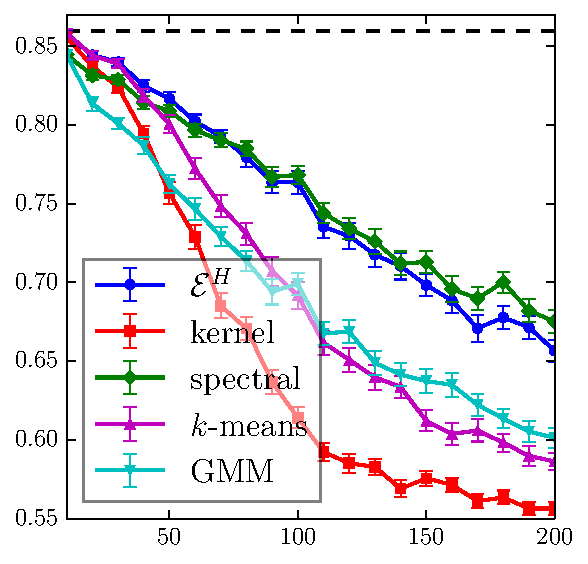
\includegraphics[scale=0.41]{normal_highdim_mean.pdf}
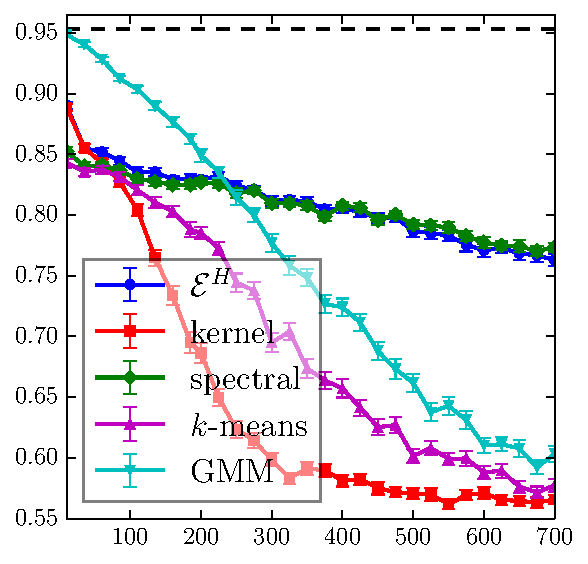
\includegraphics[scale=0.41]{normal_highdim_cov.pdf}
\put(-180,-7){(a)}
\put(-60,-7){(b)}
\caption{
\label{fig:gauss}
High dimensional Gaussian mixture.
Comparison of $\mathcal{E}^H$-clustering, kernel $k$-means, spectral
clustering, $k$-means and GMM (last three from scikit-learn).
(a) Parameters as in \eqref{eq:gauss1}. 
(b) Parameters as in \eqref{eq:gauss2}. Dashed line is Bayes accuracy.
We plot mean accuracy versus number of dimensions $D$ over $100$ Monte
Carlo trials, error bars are standard error.
}
\end{figure} 

First we analyze
how the algorithms degrade as the number of dimensions increase while
keeping Bayes error fixed.
Consider data from a Gaussian mixture
$x  \stackrel{iid}{\sim} 
\tfrac{1}{2}\left[\mathcal{N}(\mu_1,\Sigma_1) +
\mathcal{N}(\mu_2,\Sigma_2)\right]$ in $\mathbb{R}^D$ with
$\Sigma_1=\Sigma_2 = I_D$,   
\begin{equation}
\label{eq:gauss1}
\mu_1 = (\underbrace{0,\dotsc,0}_{\times D})^\top, \
\mu_2 = 0.7 (\underbrace{1,\dots,1}_{\times 10},
\underbrace{0,\dots,0}_{\times (D-10)})^\top.
\end{equation}
The Bayes error gives an optimal accuracy
$\approx 0.86$, which is fixed as $D$ increases.
We sample $200$ points for each trial.
The results are shown in Fig.~\ref{fig:gauss}a, where
$\mathcal{E}^H$- and spectral-clustering have close
performance,  
much better than kernel $k$-means, and also 
better than 
$k$-means and GMM. The improvement is noticeable in 
higher dimensions.
Still for a two-class Gaussian mixture we now choose
different numbers for the  diagonal covariance $\Sigma_2$.
We have $\Sigma_1=I_D$, $\mu_1=(0,\dotsc,0)^\top \in \mathbb{R}^D$,
$\mu_2=(1,\dotsc,1,0,\dotsc,0)^T \in \mathbb{R}^D$ 
with signal in the first $10$ dimensions, and
\begin{equation}
\label{eq:gauss2}
\begin{split}
\Sigma_2 &= \left( \begin{array}{c|c}
\widetilde{\Sigma}_{10} & 0 \\ \hline 
0 & I_{D-10} \end{array}\right), \\
\widetilde{\Sigma}_{10} &= \diag(1.367,  3.175,  3.247,  4.403,  1.249,\\
&\hspace{3.6em}1.969, 4.035,   4.237,  2.813,  3.637).
\end{split}
\end{equation}
We simply chose $10$ number uniformly at random on the interval
$[1,5]$, and any other choice would give analogous results.
The Bayes  accuracy is fixed at $\approx 0.95$.
Fig.~\ref{fig:gauss}b we show the results. 
GMM performs better in low dimensions, 
but it quickly degenerates
as $D$ increases, as (kernel) $k$-means, while  
$\mathcal{E}^H$- and spectral-clustering remains much more stable. 

\begin{figure}[t]
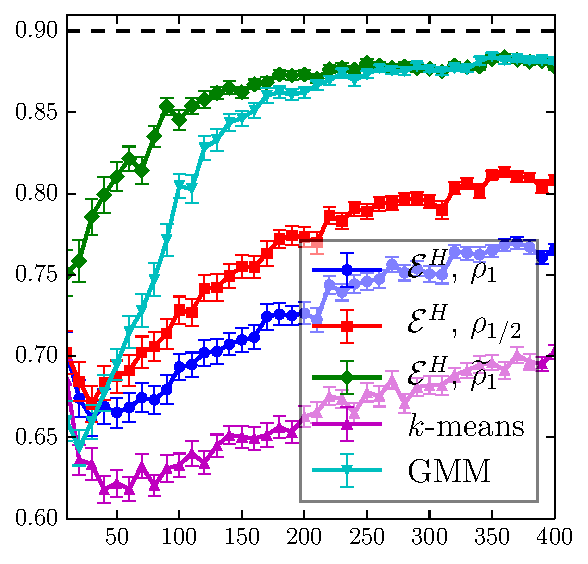
\includegraphics[scale=.41]{normal_kernels.pdf}
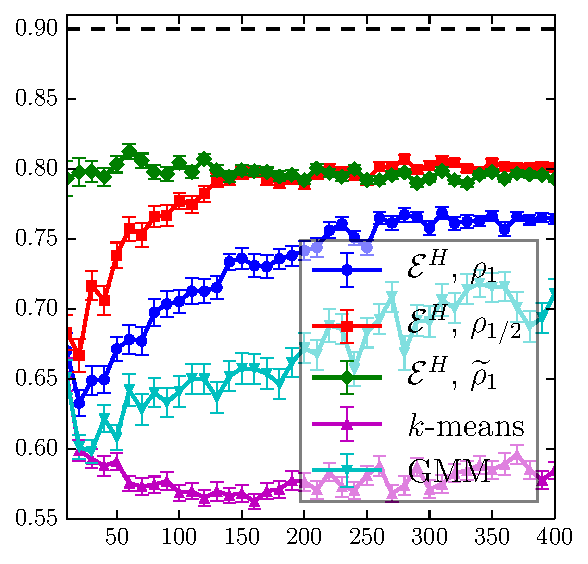
\includegraphics[scale=.41]{lognormal_kernels.pdf}\\
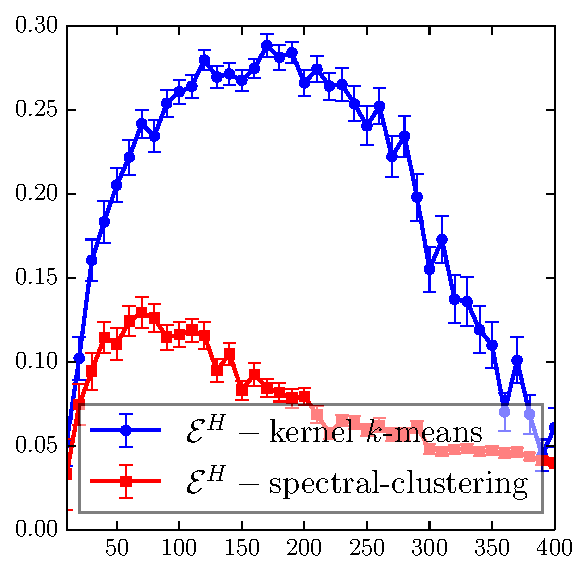
\includegraphics[scale=.41]{normal_kernels_difference.pdf}
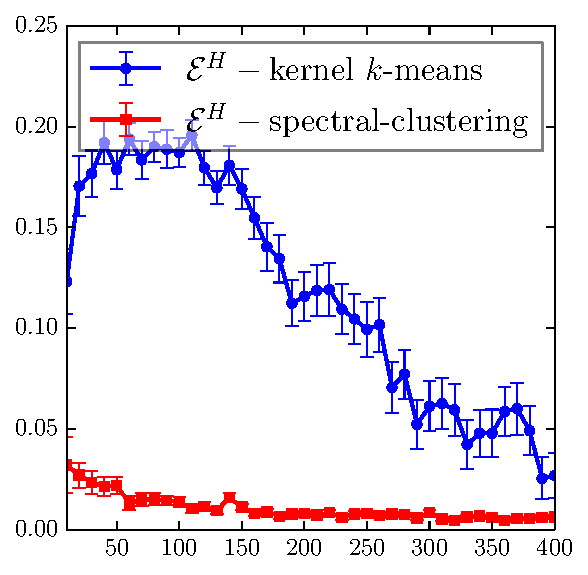
\includegraphics[scale=.41]{lognormal_kernels_difference.pdf}
\put(-180,117){(a)}
\put(-60,117){(c)}
\put(-180,-10){(b)}
\put(-60,-10){(d)}
\caption{
\label{fig:consist}
(a,b) Normal and (c,d) lognormal distributions in $\mathbb{R}^{20}$ with
parameters \eqref{eq:20gauss}. We use different kernels
for $\mathcal{E}^H$-clustering, compared to 
$k$-means and GMM. Bayes accuracy
is $\approx 0.9$. We plot average accuracy (error bars are standard error)
versus number of points for $100$ Monte Carlo trials.
The plots in (c) and (d) consider the difference in accuracy
between $\mathcal{E}^H$ versus kernel $k$-means and
spectral clustering, with $\widetilde{\rho}_1$.
}
\end{figure}


Now we sample $n$ points from the Gaussian mixture
$x \stackrel{iid}{\sim} \tfrac{1}{2}\left[ \mathcal{N}(\mu_1,\Sigma_1)+
\mathcal{N}(\mu_2, \Sigma_2) \right]$ in $\mathbb{R}^{20}$ with 
$\Sigma_1=\tfrac{1}{2} I_{20}$, $\Sigma_2 = I_{20}$, 
\begin{equation}
\label{eq:20gauss}
\mu_1 = (\underbrace{0,\dotsc,0}_{\times 20})^\top ,\quad
\mu_2 = \tfrac{1}{2} 
(\underbrace{1,\dotsc,1}_{5},\underbrace{0,\dotsc,0}_{15})^\top.
\end{equation}
Bayes accuracy is $\approx 0.90$. 
We increase the sample size in the range $n \in [10, 400]$. 
The results are 
shown in Fig.~\ref{fig:consist}a, where we compare
$\mathcal{E}^H$-clustering with different
kernels, indicated in the legend, to $k$-means and GMM.
%For small $n$ all methods
%are superior than GMM, which eventually catches up and tend to optimal Bayes,
%as expected since it is consistent to this setting. 
Note that $\mathcal{E}^H$-clustering
with $\widetilde{\rho}_1$ is as accurate as GMM for large number of points, 
however, it is superior for small number of points. Still for
the same setting, in Fig.~\ref{fig:consist}b we
we show the difference in accuracy provided by $\mathcal{E}^H$ minus
kernel $k$-means and $\mathcal{E}^H$ minus spectral clustering, when using the
semimetric $\widetilde{\rho}_1$.
Note that $\mathcal{E}^H$ was
always superior (there would be points with negative values on 
the $y$-axis otherwise).
Now consider the same parameters as in \eqref{eq:20gauss} but with
lognormal mixtures in $\mathbb{R}^D$,
$\log x \stackrel{iid}{\sim} \tfrac{1}{2}\left[ \mathcal{N}(\mu_1,\Sigma_1)+
\mathcal{N}(\mu_2, \Sigma_2) \right]$. 
The same experiments are shown in 
Fig.~\ref{fig:consist}c and Fig.~\ref{fig:consist}d.
Note that $\mathcal{E}^H$-clustering still performs accurately, 
with any of those
kernels, providing better results than $k$-means and GMM. 
%The semimetric $\widetilde{\rho}_1$ still provides the 
%best results for small number of points, but its performance is eventually 
%achieved by $\rho_{1/2}$, indicating that $\alpha \approx 1/2$ in the standard
%energy distance should be more appropriate for skewed distributions.
These two experiments
illustrate how energy clustering is flexible,
since it is accurate on data from very different distributions
with the same kernel. 

\begin{figure}[t!]
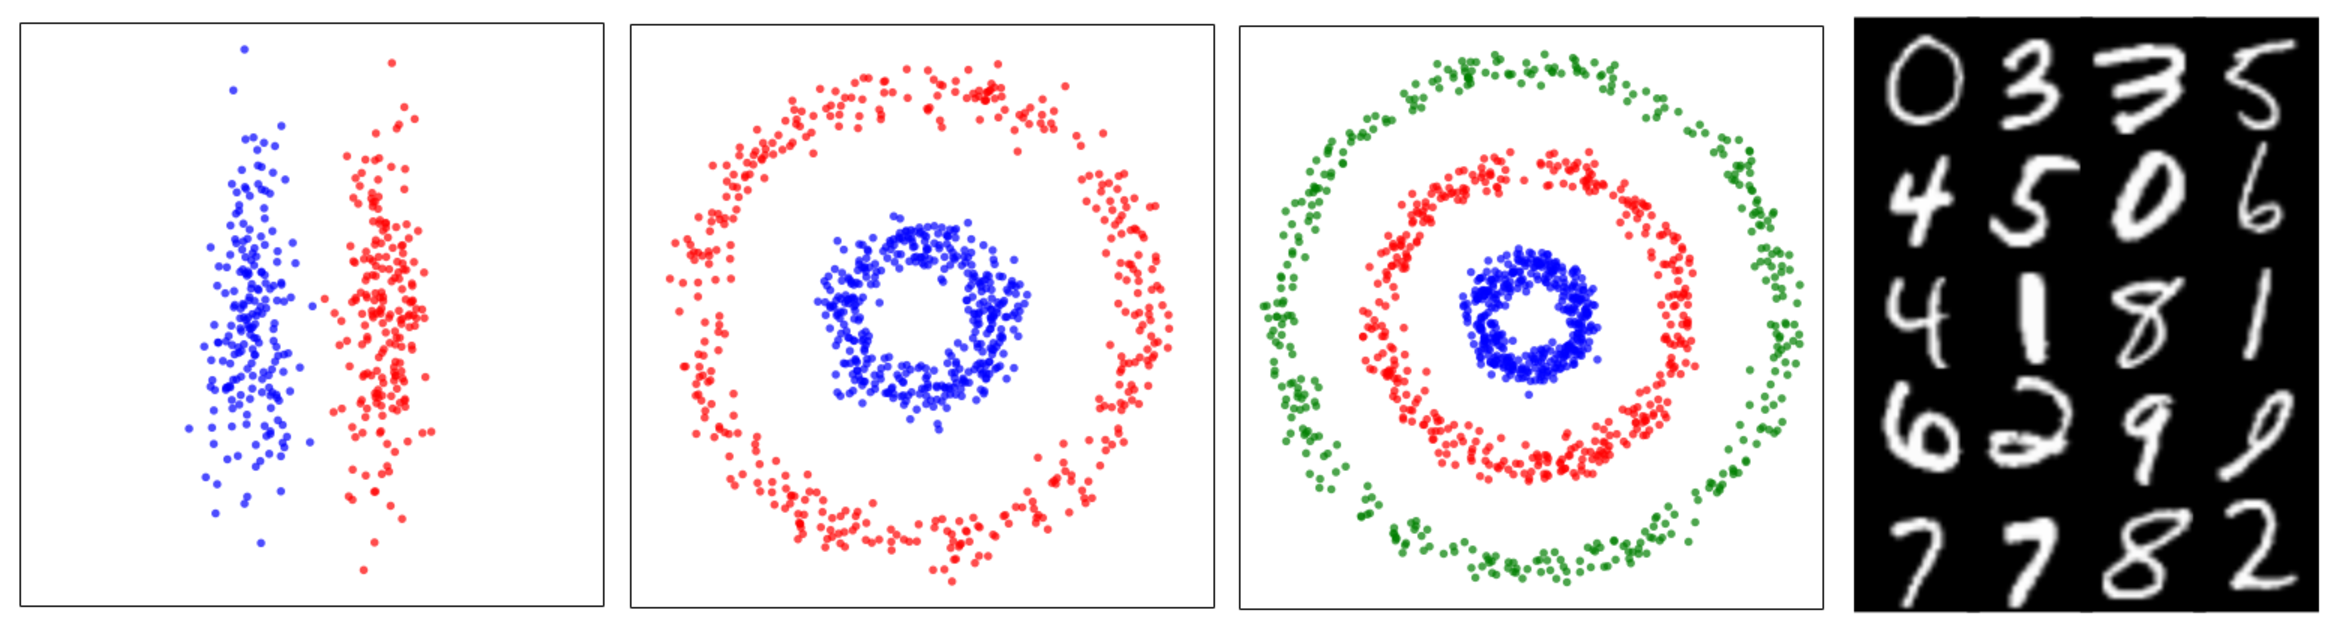
\includegraphics[scale=0.21]{complex_data.pdf}
\put(-210,-10){(a)}
\put(-150,-10){(b)}
\put(-90,-10){(c)}
\put(-35,-10){(d)}
\caption{\label{fig:other}
(a) Parallel cigars, $200$ points each. (b,c) Two and three  
concentric circles with Gaussian noise, $400$ points each.   
(d) MNIST handwritten digits.
Clustering results are in Tables~\ref{table:other} and
\ref{table:mnist}.
}
\end{figure}




\begin{table*}
\caption{\label{table:other}
Clustering data from Fig.~\ref{fig:other}a--c.
}
\begin{center}
%\footnotesize{
\begin{tabular}{@{}r|  l l  l l  l l@{}}
\toprule[1pt]
 & & \emph{Fig.~\ref{fig:other}a}
 & & \emph{Fig.~\ref{fig:other}b}
 & & \emph{Fig.~\ref{fig:other}c} \\
\midrule[0.5pt]
\multirow{4}{*}{\emph{$\mathcal{E}^H$-clustering~~~~}}
& $\rho_{1}$ & $0.705\pm 0.065$
& $\rho_{1}$ & $0.521\pm 0.005$
& $\rho_{1}$ & $0.393\pm 0.020$ \\
& $\rho_{1/2}$ & $0.952\pm 0.048$
& $\rho_{1/2}$ & $0.522\pm 0.004$
& $\rho_{1/2}$ & $0.486\pm 0.040$ \\
& $\widetilde{\rho}_{2}$ & $\bm{0.9987\pm 0.0008}$
& $\widetilde{\rho}_{1}$ & $0.778\pm 0.075$
& $\widetilde{\rho}_{2}$ & $0.666\pm 0.007$ \\
& $\widehat{\rho}_{2}$  & $0.956\pm 0.020$
& $\widehat{\rho}_{1}$  & $\bm{1.0\pm 0.0}$
& $\widehat{\rho}_{2}$ & $\bm{0.676\pm 0.002}$ \\
\midrule[0.5pt]
\emph{spectral-clustering~~~~}
& $\widetilde{\rho}_{2}$ & $0.557\pm 0.014$ 
& $\widehat{\rho}_{1}$ & $0.732\pm 0.002$ 
& $\widehat{\rho}_{2}$ & $0.364\pm 0.004$  \\
\emph{$k$-means}~~~~ 
& \xmark & $0.550\pm 0.011$
& \xmark & $0.522\pm 0.004$
& \xmark & $0.368\pm 0.005$ \\
\emph{GMM}~~~~
& \xmark & $0.903\pm 0.064$
& \xmark & $0.595\pm 0.011$
& \xmark & $0.465\pm 0.030$ \\
\bottomrule[1pt]
\end{tabular}
%}
\end{center}
\end{table*}

\begin{table*}
\caption{\label{table:mnist}
Clustering MNIST data from Fig.~\ref{fig:other}d.
}
\begin{center}
%\footnotesize{
\begin{tabular}{@{}r@{}l@{}|@{}l@{}|@{}l@{}|@{}l@{}|@{}l@{}}
\toprule[1pt]
\emph{Class Subset}~~~~ & & 
$~\{0,1,2\}$ &
$~\{0,1,\dotsc,4\}~$ &
$~\{0,1,\dotsc,6\}~$ &
$~\{0,1,\dotsc,8\}~$ \\
parameter~~~~ & {$\sigma$}
& $~10.34~$
& $~10.41~$
& $~10.41~$
& $~10.37~$ \\
\midrule[0.5pt]
\multirow{3}{*}{\emph{$\mathcal{E}^H$-clustering~~~~}}
& $\rho_{1}$\hspace{1em} 
&$~0.937\pm 0.006~$
&$~0.873\pm 0.025~$
&$~0.731\pm 0.016~$
&$~0.687\pm 0.016~$
\\
& $\rho_{1/2}$ 
&$~0.939\pm 0.006~$
&$~0.874\pm 0.027~$
&$~0.722\pm 0.017~$
&$~0.647\pm 0.017~$
\\
& $\widetilde{\rho}_{\sigma}$ 
&$~0.939\pm 0.006~$
&$~0.847\pm 0.031~$
&$~0.695\pm 0.023~$
&$~0.657\pm 0.014~$
\\
& $\widehat{\rho}_{\sigma}$ 
&$~0.933\pm 0.005~$
&$~\bm{0.891\pm 0.009}~$
&$~\bm{0.759\pm 0.011}~$
&$~\bm{0.704\pm 0.011}~$
\\
\midrule[.5pt]
\emph{spectral-clustering~~~~} 
& $\widehat{\rho}_{\sigma}$ 
&$~0.823\pm 0.015~$
&$~0.769\pm 0.012~$
&$~0.678\pm 0.014~$
&$~0.649\pm 0.018~$
\\
\emph{$k$-means}~~~~ & \xmark
&$~0.927\pm 0.004~$
&$~0.878\pm 0.010~$
&$~0.744\pm 0.008~$
&$~0.695\pm 0.012~$
\\
\emph{GMM}~~~~ & \xmark
&$~\bm{0.952\pm 0.005}~$
&$~0.839\pm 0.015~$
&$~0.694\pm 0.010~$
&$~0.621\pm 0.009~$
\\
\bottomrule[1pt]
\end{tabular}
%}
\end{center}
\end{table*}

In Fig.~\ref{fig:other}a--c we have 
complex two dimensional datasets. 
We apply $\mathcal{E}^H$-clustering  with different kernel choices.
We also consider the best kernel choice for spectral
clustering, besides 
$k$-means and GMM. Here we perform only $10$ Monte Carlo runs.
In (a) we initialize
all algorithms with $k$-means++, and in (b) and (c) we initialize at
random.
The results are in Table~\ref{table:other}.
$\mathcal{E}^H$-clustering has superior performance
in every example, and in particular better than the
spectral clustering.
For the data in Fig.~\ref{fig:other}a 
the semimetrics $\rho_1$ and $\rho_{1/2}$ still provide
accurate results, however, for the
examples in (b) and (c) the kernel choice is more sensitive.


Next, we consider 
the infamous MNIST handwritten digits
as illustrated in Fig.~\ref{fig:other}d.
Each data point is an $8$-bit gray scale
image forming a $784$-dimensional vector 
corresponding to the digits $\{0,1,\dotsc,9 \}$.
We compute the parameter 
\begin{equation}
\label{eq:sigma}
\sigma^2 = \dfrac{1}{n^2} \sum_{i,j=1}^n \| x_i - x_j \|^2 
\end{equation}
from a separate
training set, to be used in the kernels.
We consider subsets of $\{0,1,\dotsc,9 \}$, 
sampling $100$ points 
for each class over $10$ Monte Carlo trials.
The results are shown in Table~\ref{table:mnist}.
Unsupervised clustering on MNIST without any feature extraction
is not trivial. This 
same experiment was performed in \citep{Sapiro} where a low-rank
transformation is learned then subsequently used in subspace clustering. 
It would be interesting to explore methods
for learning a better representation of the data and subsequently apply
$\mathcal{E}^H$-clustering.


%%%%%%%%%%%%%%%%%%%%%%%%%%%%%%%%%%%%%%%%%%%%%%%%%%%%%%%%%%%%%%%%%%%%%%%%%%%%%%%
\section{Discussion}
\label{sec:conclusion}

We considered clustering from the perspective of generalized energy
statistics, valid for arbitrary spaces of negative type.
Our mathematical formulation of energy clustering 
reduces to a QCQP in the associated RKHS, as demonstrated in 
Proposition~\ref{th:qcqp2}.
We showed that the optimization problem
is equivalent
to kernel $k$-means, once the kernel is fixed; see
Proposition~\ref{th:kernel_kmeans}. Energy statistics, however, fixes
a family of standard kernels in Euclidean space, and
more general kernels 
on spaces of negative type can also be obtained.
We proposed the iterative $\mathcal{E}^H$-clustering algorithm based on 
Hartigan's method, which was compared to kernel $k$-means algorithm
based on Lloyd's heuristic.
Both have the same time complexity, however, numerical and theoretical
results provide compelling evidence that $\mathcal{E}^H$-clustering
is more robust with a superior performance, specially in high
dimensions. 
Furthermore, energy clustering, with standard kernels from energy
statistics, outperformed $k$-means and GMM
on several settings, even on Gaussian ones, illustrating the flexibility
of the proposed method. In some
examples the iterative
$\mathcal{E}^H$-clustering also surpassed spectral clustering, and in
others performed similarly but never worse.

A limitation of $\mathcal{E}^H$-clustering  is that it cannot
handle accurately highly unbalanced clusters. 
An interesting problem would be to
extend $\mathcal{E}^H$-clustering to these cases.
Moreover, it would also be interesting to formally 
demonstrate cases where energy clustering is a 
consistent. A soft version of energy clustering is also an
interesting extension.
Finally, kernel methods can benefit from sparsity and
fixed-rank approximations of the Gram matrix, and there is plenty
of room to make $\mathcal{E}^H$-clustering algorithm more scalable.


\subsection*{Acknowledgements}
We would like to thank Carey Priebe for discussions.
This work was supported by NIH TRA grant.


%\bibliographystyle{unsrt}
%\bibliographystyle{plainnat}
\bibliographystyle{abbrvnat}
\bibliography{biblio.bib}

\clearpage

\appendix

\section{Supplementary Material}

Here we colect the proofs of our main results.

\begin{proof}[Proof of Lemma~\ref{th:minimize}]
From \eqref{eq:within} and \eqref{eq:between}
we have
\begin{equation}
\begin{split}
S + W &= 
\dfrac{1}{2n} \sum_{\substack{i,j=1 \\ i\ne j}}^k n_i n_j g(\C_i, \C_j)
\\&+ \dfrac{1}{2n} \sum_{i=1}^{k} 
\bigg[ n - 
\sum_{j\ne i = 1}^k n_j \bigg] 
n_i g(\C_i, \C_i) \\
& = \dfrac{1}{2n} \sum_{i,j=1}^k n_i n_j g(\C_i, \C_j) \\
&= \dfrac{1}{2n} \sum_{x \in \mathbb{X}} \sum_{y \in \mathbb{X}} \rho(x,y)\\
&= \dfrac{n}{2} g(\mathbb{X}, \mathbb{X}).
\end{split}
\end{equation}
Note that the right hand side of this equation 
only depends on the pooled data, so it is a constant
independent of the choice of partition. Therefore, maximizing
$S$ over the choice of partition is equivalent to minimizing $W$.
\end{proof}

\begin{proof}[Proof of Proposition~\ref{th:qcqp2}]
From 
\eqref{eq:gen_kernel},
\eqref{eq:g_def}, and
\eqref{eq:within}
we have
\begin{equation}
\label{eq:W2}
\begin{split}
W
&= \dfrac{1}{2} \sum_{j=1}^k \dfrac{1}{n_j} \sum_{x,y \in \C_j} \rho(x,y) \\
&= \sum_{j=1}^k \sum_{x \in \C_j}  \bigg(
\kk(x,x) - \dfrac{1}{n_j} \sum_{y \in \C_j} \kk(x,y) \bigg).
\end{split}
\end{equation}
Note that the first term is global so it does not contribute to the 
optimization problem.
Therefore, minimizing \eqref{eq:W2} is equivalent to
\begin{equation}
\label{eq:max_prob}
\max_{ \C_1,\dotsc,\C_k } 
\sum_{j=1}^k \dfrac{1}{n_j} \sum_{x,y\in C_j} \kk(x,y) .
\end{equation}
But 
\begin{equation}
\sum_{x, y \in \C_j} \kk(x, y) =
\sum_{p=1}^{n} \sum_{q=1}^{n} Z_{pj} Z_{qj} G_{pq} = 
(Z^\top G \, Z)_{jj},
\end{equation}
where we used the definitions \eqref{eq:kernel_matrix} and
\eqref{eq:label_matrix}. 
Notice that $n_j^{-1} = D^{-1}_{jj}$, where the diagonal matrix $D = 
\diag(n_1,\dotsc,n_k)$ contains the number of points in each cluster, 
thus the objective function in 
\eqref{eq:max_prob} is equal to $\sum_{j=1}^k D^{-1}_{jj} 
\left( Z^\top G Z \right)_{jj} = \Tr \left( D^{-1} Z^\top G Z \right)$. 
Now we can
use the cyclic property
of the trace, and by the  definition of the matrix $Z$
in \eqref{eq:label_matrix}, we obtain the following integer
programing problem:
\begin{equation}\label{eq:qcqp}
\begin{split}
&\max_{Z} \Tr\Big( \big( Z D^{-1/2}\big)^\top G 
\big( ZD^{-1/2} \big) 
\Big) \\
&\mbox{s.t. $Z_{ij} \in \{0,1\}$, $\sum_{j=1}^k Z_{ij} = 1$, 
$\sum_{i=1}^n Z_{ij} = n_j$.}
\end{split}
\end{equation}

Now we write this in terms of the matrix $Y = Z D^{-1/2}$.
The objective function immediately becomes
$\Tr\left( Y^\top G \, Y\right)$. Notice that the above constraints
imply that $Z^T Z = D$, which in turn gives
$D^{-1/2} Y^T Y D^{-1/2} = D$, or $Y^\top Y = I$. 
Also, every entry of $Y$ is positive by definition,
$Y \ge 0$. Now it only remains to show the last 
constraint in \eqref{eq:qcqp2}, which comes from the last
constraint in \eqref{eq:qcqp}. In matrix form this reads
$Z^T \e = D \e$. Replacing $Z=YD^{1/2}$ we have
$Y^\top \e = D^{1/2} \e$. Multiplying this last equation
on the left by $Y$, and noticing
that $Y D^{1/2} \e = Z \e = \e$, we finally obtain
$Y Y^\top \e = \e$. Therefore, the optimization 
problem \eqref{eq:qcqp} is equivalent
to \eqref{eq:qcqp2} .
\end{proof}

\begin{proof}[Proof of Proposition~\ref{th:kernel_kmeans}]
Notice that 
\begin{equation}
\begin{split}
\| \varphi(x) - \varphi(\mu_j) \|^2 &= \langle 
\varphi(x),  \varphi(x) \rangle
- 2 \langle \varphi(x), \varphi(\mu_j)\rangle \\
& \qquad + \langle \varphi(\mu_j), \varphi(\mu_j) \rangle,
\end{split}
\end{equation}
therefore, kernel $k$-means objective function becomes
\begin{equation}
\label{eq:J}
\begin{split}
\sum_{j=1}^k \sum_{x\in\C_j} \bigg(
\kk(x,x) - 
\dfrac{2}{n_j} \sum_{y\in \C_j} \kk(x,y) \\
+ \dfrac{1}{n_j^2}
\sum_{y,z \in \C_j} \kk(y,z) \bigg).
\end{split}
\end{equation}
The first term is global so it does not contribute to the optimization
problem. Notice that the third term gives
$\sum_{x\in\C_j} \tfrac{1}{n_j^2} \sum_{y,z\in\C_j} \kk(y,z) =
\tfrac{1}{n_j}\sum_{y,z\in\C_j} \kk(y,z)$, which is the same as
the second term. Thus, problem
\eqref{eq:kernel_kmeans} is equivalent to
\begin{equation}
\max_{\C_1,\dotsc,\C_k}
\sum_{j=1}^k \dfrac{1}{n_j} \sum_{x,y \in\C_j} \kk(x,y) 
\end{equation}
which is exactly the same as 
\eqref{eq:max_prob} from the energy statistics formulation. Therefore,
once the kernel $\kk$ is fixed, the function 
$W$ given by \eqref{eq:within} is the same
as $J$ in \eqref{eq:kernel_kmeans}.
The remaining of the proof proceeds as 
already shown in the proof of Proposition~\ref{th:qcqp2}, leading to
the optimization problem \eqref{eq:qcqp2}.
\end{proof}

\end{document}




